\documentclass[11pt, oneside]{article}   	% use "amsart" instead of "article" for AMSLaTeX format
\usepackage{geometry}                		% See geometry.pdf to learn the layout options. There are lots.
\geometry{letterpaper}                   		% ... or a4paper or a5paper or ... 
%\geometry{landscape}                		% Activate for for rotated page geometry
%\usepackage[parfill]{parskip}    		% Activate to begin paragraphs with an empty line rather than an indent
\usepackage{graphicx}				% Use pdf, png, jpg, or eps§ with pdflatex; use eps in DVI mode
								% TeX will automatically convert eps --> pdf in pdflatex		
\usepackage{amssymb}
\usepackage{amsmath}
\usepackage{parskip}
\usepackage{color}
\usepackage{hyperref}

\title{Real Integrals}
%\author{The Author}
%\section{}
%\subsection*{}
\date{}							% Activate to display a given date or no date

\graphicspath{{/Users/telliott/Github/Tex/png/}}
% \begin{center} 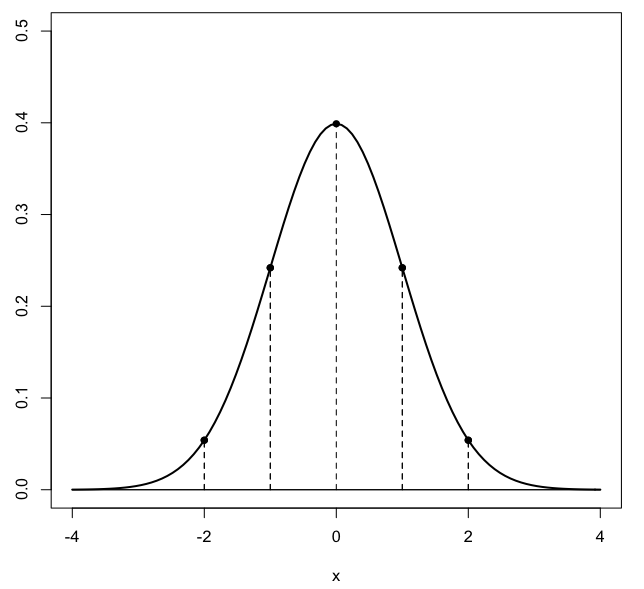
\includegraphics [scale=0.4] {gauss3.png} \end{center}
\begin{document}
\maketitle
\Large

\subsection*{inverse tangent}

Note the complex function
\[ \oint_C^{\infty} \frac{1}{1 + z^2} \ dz \]

We solved this one previously.  Basically we factor the integrand as
\[ - \frac{1}{2i} \ [ \ \frac{1}{z + i} - \frac{1}{z - i} \ ] \]

We will integrate over a path that includes only the pole at $z = i$, so only the second term contributes, and by Cauchy 2 the value is
\[ I = 2 \pi i f(z_0) = 2 \pi i \cdot (- \frac{1}{2i}) \cdot (-1) = \pi \]

Now we do the same integral on the real axis, with different limits:
\[ \int_0^{\infty} \frac{1}{1 + x^2} \ dx \]

We know the answer to this one, it is 
\[ \tan^{-1} x \ \bigg |_0^{\infty} = \frac{\pi}{2}  \]

Since $f(x)$ is an even function, the integral over $-\infty \rightarrow \infty = \pi$.

We feel there ought to be a connection between the two results:  real and complex.

Suppose we draw a different curve (contour) extending on its base from $-\infty \rightarrow \infty$: the real axis.  That integral is $\int f(z) \ dz$ but $y$ and $dy$ are both zero so it becomes just $\int f(x) \ dx$ with the result shown.

How to complete the contour?  Imagine a semicircle in the upper half-plane with $R \rightarrow \infty$.  That is, parametrize
\[ \gamma(\theta) = Re^{i\theta}, \ \ \ \theta \in [0, \pi] \]
\[ \gamma \ '(\theta) =  iRe^{i\theta} \]
The integral is
\[ \int_0^{\pi} \frac{1}{1 + R^2 e^{i2\theta}} \ i R e^{i \theta} \ d \theta \]
\[ = i \int_0^{\pi} \frac{1}{1/Re^{i \theta}  + R e^{i\theta}} \ \ d \theta \]

Now what?

We'll try to be more formal later, but just for now, it's clear that as $R \rightarrow \infty$, this integrand goes to 0.  So we have that the total integral for the complex case is equal to the integral for the real part plus this extra half-circle which is zero.

What this means is that if we had not know the result for the real integral, we could deduce it from the fact that the whole complex integral has value equal to $\pi$, and the part over this complex half-circle is zero.

\subsection*{Gaussian}

\subsection*{application of Cauchy 1}

The function we'll be working with is one we introduced before:
\[ u(x,y) =  e^{-x^2} e^{y^2} \cos 2xy \]
\[ v(x,y) = e^{-x^2} e^{y^2} (- \sin 2xy) \]
Everything will simplify pretty quickly.  Divide the path into its four parts and compute each separately:
Over $C1$, $y=0$ and $dy = 0$ so we have:
\[ \int_{C1} = \int u \ dx = \int_0^a e^{-x^2} e^{0} \cos 0 \ dx = \int_0^a e^{-x^2} \ dx \]
C2 ($x = a$, $dx = 0)$:
\[ \int_{C2} = - \int_0^b e^{-a^2} e^{y^2} (- \sin 2ay) \ dy  \]
C3 ($y = a$, $dy = 0)$:
\[ \int_{C3} = \int_a^0 e^{-x^2} e^{b^2} (\cos 2bx) \ dx  \]
C4 ($x = 0$, $dx = 0$):
\[ \int_{C4} = \int_b^0 e^{y^2} (-\sin 0) \ dy = 0 \]
So all together:
\[ \int_0^a e^{-x^2} \ dx - \int_0^b e^{-a^2} e^{y^2} (- \sin 2ay) \ dy + \int_a^0 e^{-x^2} e^{b^2} \cos 2bx \ dx = 0 \]
\[ \int_0^a e^{-x^2} \ dx = e^{-a^2} \int_0^b e^{y^2} (- \sin 2ay) \ dy + e^{b^2} \int_0^a e^{-x^2} \cos 2bx \ dx  \]
Let $a \rightarrow \infty$.  Then
\[ e^{-a^2} \rightarrow 0 \]
so the first term on the right side goes to zero and we have:
\[ \int_0^{\infty} e^{-x^2} \ dx = e^{b^2} \int_0^{\infty} e^{-x^2} \cos 2bx \ dx  \]
But we know the value of the left-hand side, it is 
\[ \int_0^{\infty} e^{-x^2} \ dx = \frac{\sqrt{\pi}}{2} \]
so
\[  \int_0^{\infty} e^{-x^2} \cos 2bx \ dx = \frac{\sqrt{\pi}}{2} \ e^{-b^2} \]
The Gaussian that we know, is a special case of this general form.

\subsection*{example}
We will develop a proof that
\[ \int_{-\infty}^{\infty} \frac{\sin x}{x} \ dx = \frac{\pi}{2} \]

Start by considering the function 
\[ f(z) = \frac{e^{iz}}{z} \]
Obviously there is a pole at the origin.

Now we consider a specially designed contour that avoids the origin by going around it clockwise in a semi-circle of radius $\epsilon$.
\begin{center} 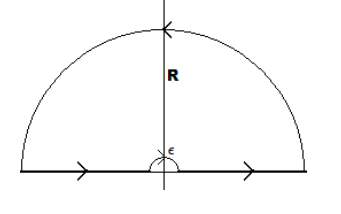
\includegraphics [scale=0.75] {contourno0.png} \end{center}
Since the integral avoids the pole, its value is zero.
\subsection*{small semi-circle}
Consider the pieces next, starting with the small semi-circle. In the limit as $\epsilon \rightarrow 0$
\[ f(z) = \frac{e^{iz}}{z} \]
\[ \text{Res }(0) = \lim_{z \rightarrow 0} z \  \frac{e^{iz}}{z} \]
\[ = \lim_{z \rightarrow 0} e^{iz} \]
\[ = 1 \]
We multiply by $\pi i$ for the half-circular path, and put in a minus sign since we are going counter-clockwise.
\[ I =  -\pi i \]

As a check write
\[ e^{iz} = \cos z + i \sin z \]
\[ = 1 - \frac{z^2}{2!} + \frac{z^4}{4!} \dots + iz - i\frac{z^3}{3!} \]
Multiply by $1/z$ to obtain
\[ = \frac{1}{z} - \frac{z}{2!} + \frac{z^3}{4!} \dots + i - i\frac{z^3}{3!} \]
In the limit $z \rightarrow 0$, 
\[ = \frac{1}{z} + i \]
Or just look at the integral term by term of the series.  The only non-zero term is
\[ \int_{\pi}^0 \frac{1}{z}  \ dz  = -\pi i \]
\subsection*{large semi-circle}
\begin{center} 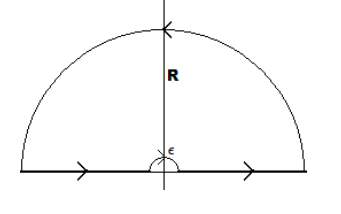
\includegraphics [scale=0.75] {contourno0.png} \end{center}
For the large semi-circle at radius $R$ we have
\[ z = Re^{i\theta} \]

\[ \int \frac{e^{iz}}{z} \ dz \]
The absolute value of the denominator is 
\[ |z| = | Re^{i\theta} | = R \]
The numerator is
\[ e^{iz} = e^{iRe^{i\theta}} \]
\[ = e^{R(i \cos \theta - \sin \theta)} \]
\[ = e^{-R \sin \theta} \ e^{R i \cos \theta} \]

Go back to the fundamental definition of length for a complex number:  $|w|^2 = ww*$.  The square of the length of the numerator is
\[ | e^{-R \sin \theta} |^2  \ [ \ e^{R i \cos \theta} e^{R(- i )\cos \theta} \ ] \]
\[ =  | e^{-R \sin \theta} |^2 \]
So the absolute value of the numerator is just
\[ e^{-R \sin \theta} \]
and the absolute value of 
\[ | \frac{e^{iz}}{z} | = \frac{e^{-R \sin \theta}}{R} \]

now 
\[ dz = Re^{i\theta} \ d \theta \]
\[ | dz | = | R d \theta | \]
so
\[ \int | \frac{e^{iz}}{z} \ dz | = \int \frac{e^{-R \sin \theta}}{R} \ R d \theta \]
\[ = \int e^{-R \sin \theta} \ d \theta \]
but in the limit as $R \rightarrow \infty$, the integrand  goes to zero.

The last two segments lie on the real axis.  The first
\[ \int_{x=-R}^{-\epsilon} \frac{e^{ix}}{x} \ dx \]
(since $y$ and $dy$ are both zero.  Now, tsubstitute $-x$ for x
\[ \int _{-x=-R}^{-\epsilon} \frac{e^{-ix}}{-x} \ d -x \]
\[ = \int _{x=R}^{\epsilon} \frac{e^{-ix}}{x} \ dx \]
the second one is just
\[ \int _{x=\epsilon}^{R} \frac{e^{ix}}{x} \ dx \]
so then in the limit as $\epsilon \rightarrow 0$ and $R \rightarrow \infty$ this is
\[ \int_0^{\infty} \frac{e^{ix}}{x} + \frac{e^{-ix}}{x} \ dx \]
\[ =  \int_0^{\infty} 2i \ \frac{\sin x}{x} \ dx \]

Adding together all four pieces and equating them to the first result for the whole contour (zero), we have
\[ 0 =  -\pi i + 0 + 2i \int_0^{\infty} \frac{\sin x}{x} \ dx  \]
Rearranging 
\[ \pi i = 2i \int_0^{\infty} \frac{\sin x}{x} \ dx  \]
\[  \int_0^{\infty} \frac{\sin x}{x} \ dx = \frac{\pi}{2}  \]

\subsection*{Complicated example using Cauchy 2}
Consider a semicircle of radius $R$ lying in the first two quadrants with its diameter on the real $x$-axis, and a function $f(z)$.   We wish to evaluate:
\[ = \oint_C \frac{e^{iaz}}{b^2 + z^2} \ dz \]
where $a$ and $b$ are positive constants.

It is apparent that $f(z)$ has singularities at $z = \pm ib$, where $b < R$.  In particular, we are interested in what happens as $R \rightarrow \infty$.

Along the $x$-axis, we have $y=0$ and $dy = 0$, so $dz = dx$ and
\[ \int_{C1} = \int_{-R}^R \frac{e^{iax}}{b^2 + x^2} \ dx \]
Along the semi-circular arc, we have $r = R$ and $\theta = 0 \rightarrow \pi$ and
\[ z = Re^{i\theta} \]
\[ dz = iRe^{i\theta} \ d \theta \]
\[ \int_{C2} = \int_0^{\pi}  \frac{e^{ia(Re^{i\theta})}}{b^2 + R^2e^{i2\theta}}  \ iRe^{i\theta} \ d \theta \]
Thus
\[ \oint_C z \ dz = \oint_C \frac{e^{iaz}}{b^2 + z^2} \ dz \]
\[ = \int_{-R}^R \frac{e^{iax}}{b^2 + x^2} \ dx + \int_0^{\pi}  \frac{e^{ia(Re^{i\theta})}}{b^2 + R^2e^{i2\theta}}  \ iRe^{i\theta} \ d \theta \]

Rewriting the integrand for the integral on the left-hand side:
\[ \frac{e^{iaz}}{b^2 + z^2} = \frac{e^{iaz}}{(z + ib)(z - ib)} = \frac{e^{iaz}}{i2b} ( \frac{1}{z-ib} - \frac{1}{z+ib}) \]
Having factored out $1/i2b$, rewrite the integral as
\[ \frac{1}{i2b} \ (\oint \frac{e^{iaz}}{z-ib} \ dz - \oint \frac{e^{iaz}}{z + ib} \ dz) = \int_{-R}^R \frac{e^{iax}}{b^2 + x^2} \ dx + \int_0^{\pi}  \frac{e^{ia(Re^{i\theta})}}{b^2 + R^2e^{i2\theta}}  \ iRe^{i\theta} \ d \theta \]
That's quite a mouthful!

The second term on the left-hand side has a singularity at $z = -ib$, which is \emph{outside} the region (actually, below it) and hence by Cauchy 1 that integral is zero.

So now
\[ \frac{1}{i2b} \ \oint \frac{e^{iaz}}{z-ib} \ dz  = \int_{-R}^R \frac{e^{iax}}{b^2 + x^2} \ dx + \int_0^{\pi}  \frac{e^{ia(Re^{i\theta})}}{b^2 + R^2e^{i2\theta}}  \ iRe^{i\theta} \ d \theta \]

Looking at the other contour integral 
\[ \frac{1}{i2b} \ \oint \frac{e^{iaz}}{z-ib} \ dz  \]

we have a singularity at $z = z_0 = ib$, which, as $R$ becomes large, is inside the semicircular region and thus by Cauchy 2 the integral is equal to $2 \pi i \ f(z_0)$ where
\[ f(z_0) = e^{iaz_0} = e^{iaib} = e^{-ab} \]
and so we have
\[ \frac{1}{i2b} \ \oint \frac{e^{iaz}}{z-ib} \ dz = \frac{1}{i2b} 2 \pi i e^{-ab}, \ \ R > b \]
\[ = \frac{\pi}{b} e^{-ab} \]

Putting it all together
\[ \frac{\pi}{b} e^{-ab} = \int_{-R}^R \frac{e^{iax}}{b^2 + x^2} \ dx + \int_0^{\pi}  \frac{e^{ia(Re^{i\theta})}}{b^2 + R^2e^{i2\theta}}  \ iRe^{i\theta} \ d \theta \]
Nahin shows that the second integral on the right-hand side vanishes as $R \rightarrow \infty$.  The reason is that we have $R^2$ in the denominator and only $R$ in the numerator.

So
\[ \frac{\pi}{b} e^{-ab} = \int_{-\infty}^{\infty} \frac{e^{iax}}{b^2 + x^2} \ dx \]\
\[ \frac{\pi}{b} e^{-ab} = \int_{-\infty}^{\infty} \frac{\cos(ax)}{b^2 + x^2} \ dx + i  \int_{-\infty}^{\infty} \frac{\sin(ax)}{b^2 + x^2} \ dx \]
The imaginary part of the left-hand side is zero, so by the equality we must have that
\[ \int_{-\infty}^{\infty} \frac{\sin(ax)}{b^2 + x^2} \ dx = 0 \]
"which is no surprise since the integrand is an odd function of $x$".  But the other result (from the real part) is:
\[ \int_{-\infty}^{\infty} \frac{\cos(ax)}{b^2 + x^2} \ dx = \frac{\pi}{b} e^{-ab} \]
In the special case $a = b = 1$ we obtain
\[ \int_{-\infty}^{\infty} \frac{\cos x }{1 + x^2} \ dx = \frac{\pi}{e} = 1.15572735 \]
which is not only an integral we didn't know how to do before, but a remarkable fraction as the result.

\end{document}  